\def\year{2018}\relax
%File: formatting-instruction.tex
\documentclass[letterpaper]{article} %DO NOT CHANGE THIS
\usepackage{aaai18}  %Required
\usepackage{times}  %Required
\usepackage{helvet}  %Required
\usepackage{courier}  %Required
\usepackage{url}  %Required
\usepackage{graphicx}  %Required
\frenchspacing  %Required
\setlength{\pdfpagewidth}{8.5in}  %Required
\setlength{\pdfpageheight}{11in}  %Required
%PDF Info Is Required:
  \pdfinfo{
/Title (2018 Formatting Instructions for Authors Using LaTeX)
/Author (AAAI Press Staff)}
\setcounter{secnumdepth}{0}  
 \begin{document}
% The file aaai.sty is the style file for AAAI Press 
% proceedings, working notes, and technical reports.
%
\title{Election Control: Attacking and Defending\\ Elections using Linear Programming}
\author{Trevor Larsen and Zach Mekus\\
Washington University in St. Louis
}
\maketitle
\begin{abstract}
For our project, we are doing an implementation of the paper Optimal Defense Against Election Control by Deleting Vote Groups by Yin et. al. The paper introduces a double oracle approach for solving the optimization problem of how to deploy defense resources to defend an election. We are implementing this double oracle algorithm, and expanding on it by applying it to each state in the 2016 election, and propose a heuristic to decide which states to attack to optimize the probability of winning a national election using the electoral college system. Current accomplishments include implenting the Attacker-MILP and Defender-MILP functions, as well as devising the heuristic we will use for maximizing probability of success over all states in an election.
\end{abstract}

\section{Introduction}
\subsection{The Problem}

In recent centuries, the majority of governments in the world have shifted to forms of government that rely on elections. In order for democratic institutions to maintain their integrity, these elections must be both free and fair, as well as protected from outside interference. Malicious attackers may have motivation to influence the outcome of an election in a certain direction by subverting the democratic process. Examples of this include attacks on voting day in 2013 in Pakistan, where bombings killed or injured over 150 people, as well as in 2010 Sri Lanka elections where there were over 250 incidents of poll-related violence. Cyber attacks on electronic voter systems are also a threat, and while no known attacks have been  in the United States, these may prove to be targets in the future, as recent investigations have found these systems to be vulnerable. 

An attacker can attack an election with the goal of either making a certain candidate the winner, which we refer to as constructive control, or to prevent a certain candidate from winning, which we call destructive control. We are interesed in the specific example of the United States presidential election, in which we will only consider the Democratic and Republican parties. In this case, making one candidate win is equivalent to making the other candidate lose, so constructive and destructive control are equivalent. In this project, we wish to investigate how we can model an attack or defense of a national presidential election in the United States, using data from the 2016 United States presidential election.

\subsection{Related Work}

The first set of prior work we will look at is papers regarding election control. The Optimal Defense paper examines the problem of protecting elections against subversion by abstracting the process of enhancing security at voting locations, either physically or electronically. Prior work included Bartholdi et al. which looked at the problem from the point of view of computational (2015) were the first to look at election control at the level of voter groups, and grouped voters by a bundling function. In the paper of Yin et al. used a function where voting groups did not overlap, and where given voting groups were deleted by the advsersary. Erdélyi et al. added or deleted voter groups in his study, but only considered constructive control.  Yin et al. in this paper was the first to consider methods for allocating defense resources for protecting given locations in an election. Elkind and Lipmaa try to make elections more difficult to subvert by developing rules that are NP-hard to manipulate, which is different from this paper, which looks at using defensive resources to reduce likelihood of an adversary changing the out come by attacking groups.

Next we will look at papers regarding physical security problems using Stackelberg games. Prior work has looked at the problem of attackers being limited to one location, whereas in Yin et al.the attackers attack multiple locations simultaneously. Other prior work has looked at simultaneous move games or have only used heuristic approaches. Other Stackelberg games have used double oracle solutions in the past, but the unique formulation of this problem requires a unique algorithm to find an optimal solution.

\subsection{Current Accomplishments}
**Zach give a short paragraph overview of current accomplishments here.**

\section{Model}
\subsection{Stackelberg Game Background}
In the following section, we introduce the concept of a Stacklberg game, which we will use in the model for our election control problem. A Stackelberg game consists of two players, a leader and a follower, who each decide on a strategy for the game. The leader goes first, picking a strategy, and the follower responds with a strategy. The strategies used can either be pure strategies, where players commit to a particular action, or a mixed strategy, where players choose a probability distribution over pure strategies. A Stackelberg security game is a model for an interaction between a defending security force and an adverserial attacker. In a Stackelberg security game, because the attacker picks second, they always are able to pick the action that gives them the highest probability of success due to their knowledge of the defender's strategy, and thus will always pick a pure strategy. In contrast, the defender doesn't have any such commitment from the attacker, and usually chooses a mixed strategy to minimize the attacker's probability of success, since the defender knows the attacker will exploit any weaknesses the defender leaves in his strategy. 

Given a defender's mixed strategy $P$ over pure strategies in $S$, $P = \{p(s) : s \in S\}$ and an attacker's action $a$ we can calculate the utility of the defender:

\begin{equation}
u^D(P,a) = \sum_{s \in S}p(s)U^D(s,a)
\end{equation}
\begin{equation}
u^A(P,a) = \sum_{s \in S}p(s)U^A(s,a)
\end{equation}

\subsection{Model of the Election}
Yin et al. model the election as a stackelberg game. The election cosists of people voting at different locations. At each location, each candidate receives a certain number of votes. Attacks are modeled as a deletion of the votes at these locations. In this model for the election, the defender is the leader, and first chooses a mixed strategy over m locations to defend,  with the goal of defending the outcome of the election. The attacker follows with a pure strategy, choosing which n locations to attack, trying to change the result of the election, either with the goal of having a specific candidate win (constructive control) or making a particular candidate lose (destructive control). 
\section{Algorithm}
Below is the general algorithm that Yin et. al suggest.
\subsection{Core-LP}
\subsection{Attack-MILP}
Yin et al. propose the following linear programming problem to solve for the attacker's optimal action given a set of potential actions and defender weak strategies.

**I think we should include the original linear program, as well as the modified constraints we used for the 2 candidate scenario.

\subsection{Defense-MILP}
\subsection{AO-Better}
\subsection{DO-Better}


\section{Results/Evaluation}

\begin{figure}
    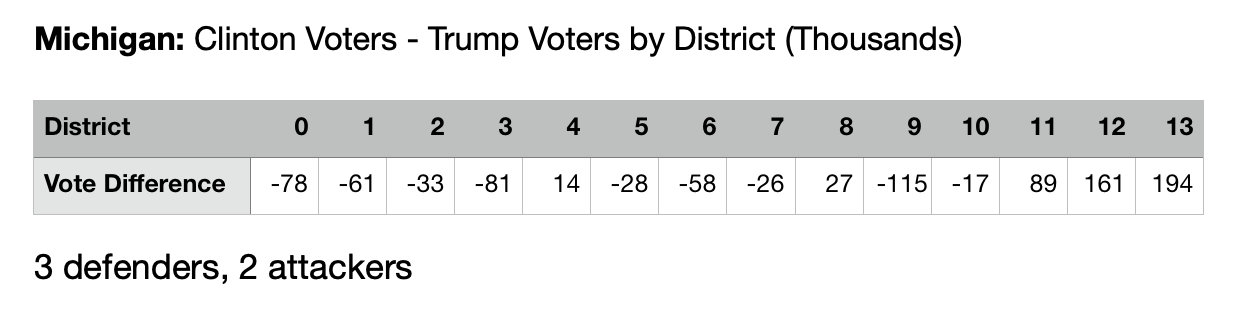
\includegraphics[width=\linewidth]{michigan_votes}
    \label{michigan_votes}
\end{figure}

\begin{figure}
    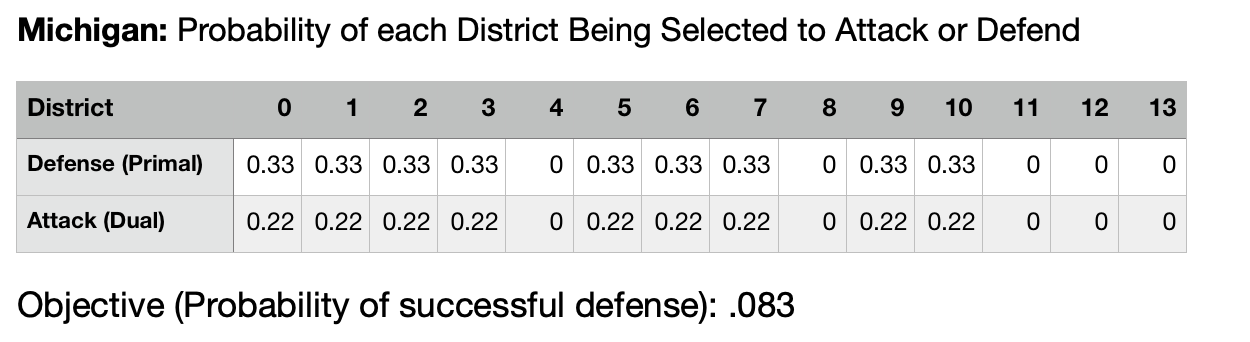
\includegraphics[width=\linewidth]{michigan_probs}
    \label{michigan_probs}
\end{figure}

\begin{figure}
    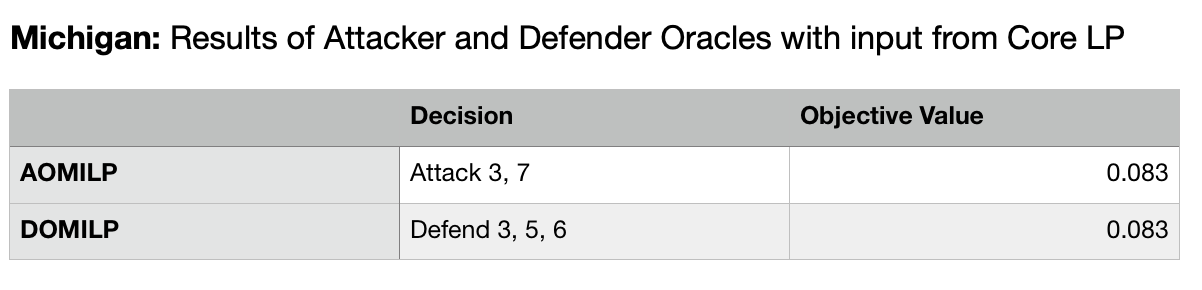
\includegraphics[width=\linewidth]{michigan_oracles}
    \label{michigan_oracles}
\end{figure}

\begin{figure}
    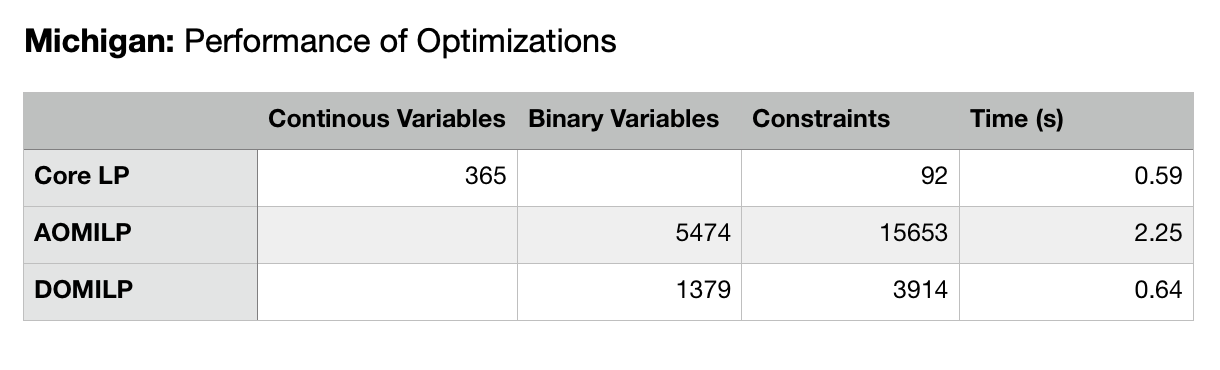
\includegraphics[width=\linewidth]{michigan_perfs}
    \label{michigan_perfs}
\end{figure}

\begin{figure}
    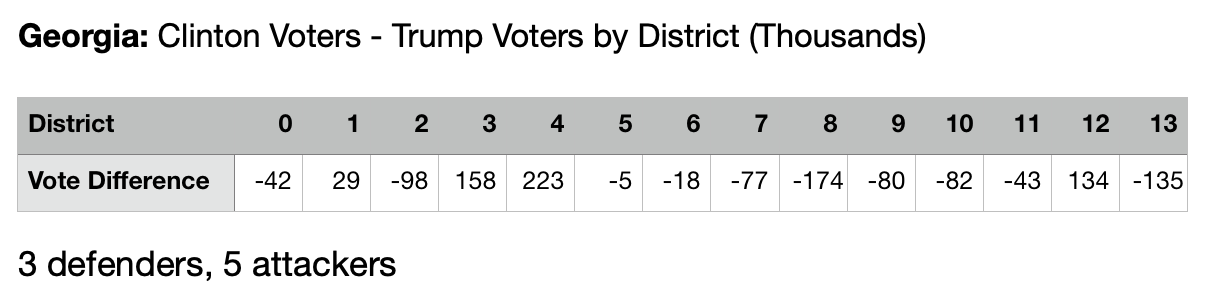
\includegraphics[width=\linewidth]{georgia_votes}
    \label{georgia_votes}
\end{figure}

\begin{figure}
    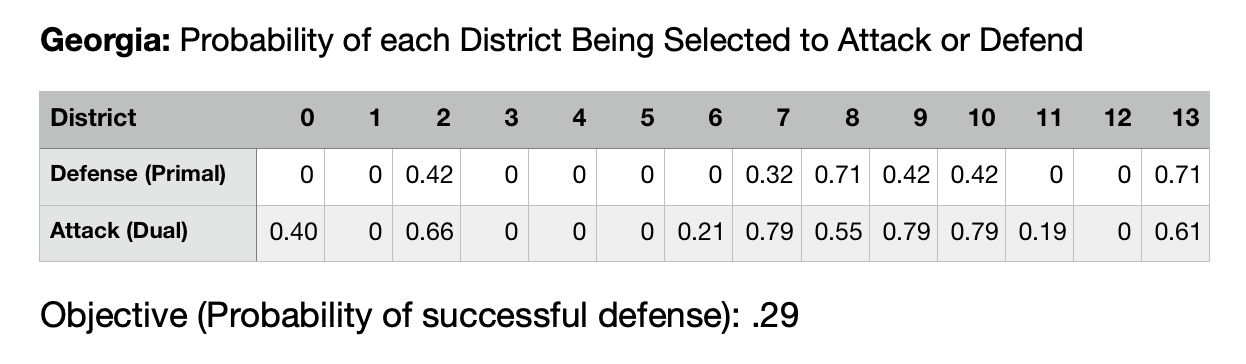
\includegraphics[width=\linewidth]{georgia_probs}
    \label{georgia_probs}
\end{figure}

\begin{figure}
    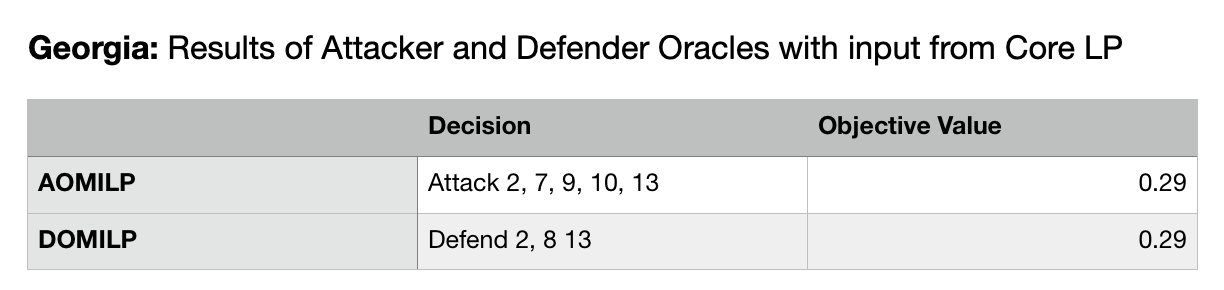
\includegraphics[width=\linewidth]{georgia_oracles}
    \label{georgia_oracles}
\end{figure}

\begin{figure}
    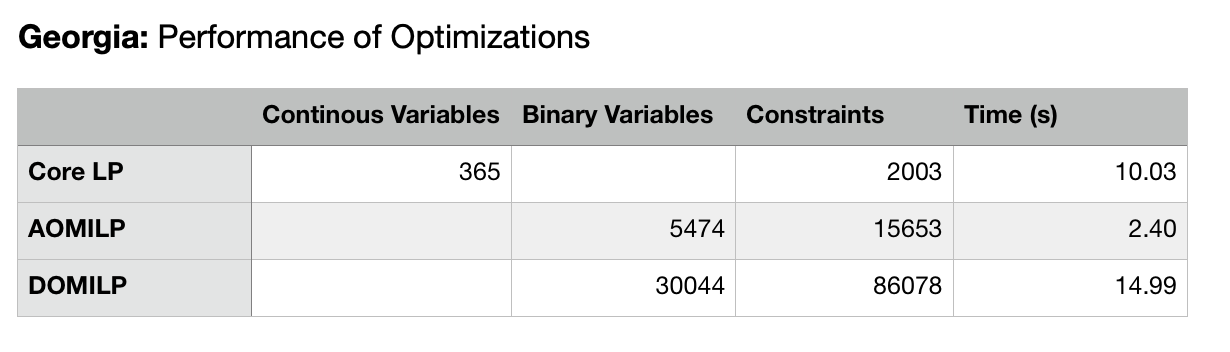
\includegraphics[width=\linewidth]{georgia_perfs}
    \label{georgia_perfs}
\end{figure}

\subsection{Overview}

The results section has the following goals: To show that what has been implemented so far is correct, to get an initial evaluation of our states data, and to gage the limitations of Core LP in terms of run time on further state data. We evaluate on 2016 US presidential election data using the difference in votes between Hillary Clinton and Donald Trump each congressional district of the states Michigan and Georgia. The optimal randomized defensive strategy is solved using Core LP and the dual solution of Core LP is the optimal randomized attacking strategy for the scenario where the attacker moves first and the defender plays a pure strategy. AOMILP and DOMILP work by taking randomized strategies and returning the optimal attacking and defending strategy respectively. To ensure these will work later on in the double oracle, these are tested here to make sure they give correct strategies and objective values. The probability vectors over the districts are calculated by finding the expectation that each district will be defended or attacked based on the randomized strategy.

\subsection{Michigan}

In 2016 the presidential election results went narrowly to Donald Trump. If any district that favored Trump is deleted, the results would have changed. Here we use three defenders and two attackers, but the results would have been similar no matter what. Since every district is equally valuable, the defenders and attackers pretect them equally. Table \ref{michigan_probs} shows the equal distribution among districts the defender won, in both the attacking and defending solutions (defending sums to 3, attacking sums to 2). This is also seen in the response in table \ref{michigan_oracles} by the attacker and defender, which arbitrarily choose districts among those the defender won. 

\subsection{Georgia}

While Georgia was competitive, it wasn't so close that any To induce a more interesting result, 3 defenders and 5 attackers were introduced and this resulted in a 29\% chance of defending successfully. As seen in table \ref{georgia_probs} the larger defender-won districts got more defense and attack. Because the attackers had more options, they could sometimes attack districts never defended. Table \ref{georgia_oracles} shows that each of the oracles corresponds to choosing the most attacked/defended districts, but not neccessarily the ones with the most votes to destroy. 


\section{Related Work}

We experiment on the same data as Yin et al. with 2016 Michigan presidential data. With the same settings, three defense and two attack resources, we both get the same result of .29 success rate. This is promising as it serves as further confirmation that we have implemented Core LP corectly. In the Results section, we expand on the choices made by the defensive and attacking agents in Michigan and Georgia to further understand the process. In the future, we hope to expand on the solving this problem for all states. 

\section{Conclusion, Limitations, and Future Work}


\begin{quote}
\begin{scriptsize}\begin{verbatim}
%References and End of Paper
%These lines must be placed at the end of your paper
\bibliography{Bibliography-File}
\bibliographystyle{aaai}
\end{document}
\end{verbatim}\end{scriptsize}
\end{quote}





\end{document}
